\section{Résumé}
Because I kind of gave up taking note in FDS, I'll just do a big summary what is needed to know.

\subsubsection{Sequential circuit}

\begin{parag}{Register}
    One flip-flop stores \textbf{one} bits of information, to store $n$ bits of information we need $n$ flip flop.\\
    An $n$ bits structures consisting of flip flops are commonly referred as \important{registers}.\\
    \begin{itemize}
        \item Clock (CLK) is common for all FFS
        \item reset (CLR) is common for all FFS
    \end{itemize}
    Common in the sense of the same
    \begin{framedremark}
    An  $n$ bits register have $2^n$ different state possible, the output of a $n$ register is a $n$ binary vector.
    \end{framedremark}
    
    \begin{subparag}{A Register in verilog}
        
    
    \begin{lstlisting}
module regn (D, CLK, CLR, Q);
    parameter n = 16; // 16 as an example
    input[n-1: 0] D;
    input CLK, CLR;
    output reg [n-1:0] Q];

    always  (posedge CLK)
    begin
    if (CLR == 1) // synchronous reset
        Q <= 0;
    else
        Q <= D;
    end
endmodule   
    \end{lstlisting}
    
    \begin{itemize}
        \item $n$ instances of DFFs, taking a vector $D$ and producing a vector $Q$:
            \begin{align*} Q\left[i\right] =  D\left[i\right] \end{align*}
            \item Recall: Parameters associate an identifier name with a constant
                \begin{itemize}
                    \item Here, the parameter $n$ serves just as a constant, which is the number of FFs in the register
                \end{itemize}
                
    \end{itemize}
    \end{subparag}
\end{parag}
\begin{parag}{Shift registers}
    A shift register \textbf{shift} their $n$ bits value one bit to the left or right:
    \begin{itemize}
        \item Take $1$ bit input (serial) or, sometimes $n$-input (parallel)
        \item Produce $1$ bits output (serial) or $n$-bits output (parallel)
    \end{itemize}
    This is used in a variety of applications: Serial to parallel conversion, data storage, arithmetic, frequency division...
    
    
\end{parag}


\begin{parag}{Example}
    We need $n$ FFs, the circuit below performs shift right\\
    $1$ bits input $IN$ arrives at the $1$ bit output $OUT$ after $n$ clock cycles (here $n = 4$)
    \begin{center}
        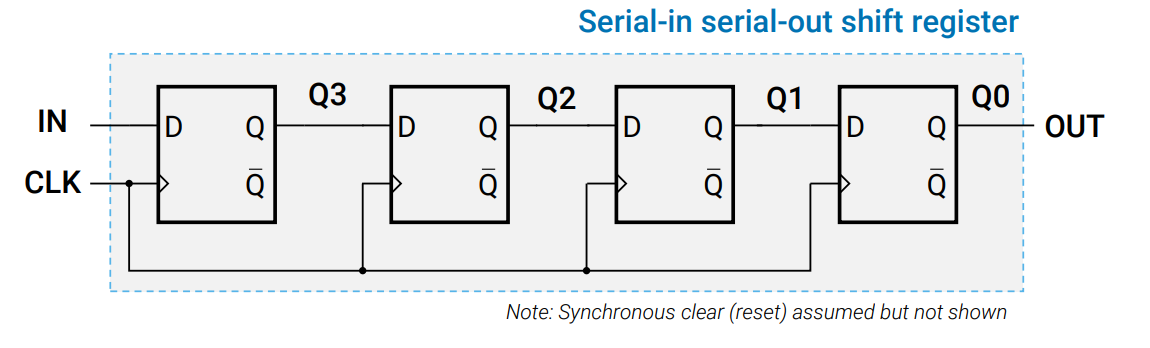
\includegraphics[scale=0.3]{42025-06-20.png}
    \end{center}
    For instance if we take such that $Q_i = 0 \mathspace \forall i =0, \ldots 3$ and that we input for each clock cycle $1$ or $0$ we have:
    \begin{center} \begin{tabular}{c|c|cccc}$t_i$ & $IN$ & $Q_3$ & $Q_2$ & $Q_1$ & $Q_0$($OUT$) \\   \hline
 $t_0$ & 1 & 0 & 0 & 0 & 0 \\ $t_1$ & 0 & 1 & 0 & 0 & 0 \\ $t_2$ & 1 & 0 & 1 &0  &0  \\$t_3$   & 1 &1  &0  &1  &0  \\ $t_4$ &1  &1  &1  & 0 & 1 \\ $t_5$ &0  & 1 &1  &1  &0  \\$t_6$  & 0 & 0 & 1 & 1 &1 \\
    $t_7$ &0 & 0 & 0 & 1 & 1  \end{tabular} \end{center} 
    Is we take then the verilog code:
    \begin{lstlisting}
module shiftn( IN, CLR, CLK, OUT);
    parameter n = 4; // 4 bits shifter
    input IN, CLR, CLK;
    output OUT;

    reg [n-1:0] Q; // Internal

    always @ (posedge CLK)
    begin
    if (CLR == 1) Q <= 0; // Reset of the register
    else Q <= {IN, Q[n-1:1]}; // trunced the register
    
    assign out = Q[0];
endmodule    
    \end{lstlisting}
    Here the ``tricky'' part is to use the syntax of verilog which allows us the add together value as seen here
    
    
    
\end{parag}


\begin{parag}{Shift right parallel}
    Here, we just do the same thing as before, but we want to add the possibility to  also load data in parallel when wanted, we use one value $SEL$ which let us know which one to chose (shift one bit, or load $D$) Furthermore, we also want to have access at every $Q_i$ not just the last one, therefor the output will be $Q$
    \begin{center}
        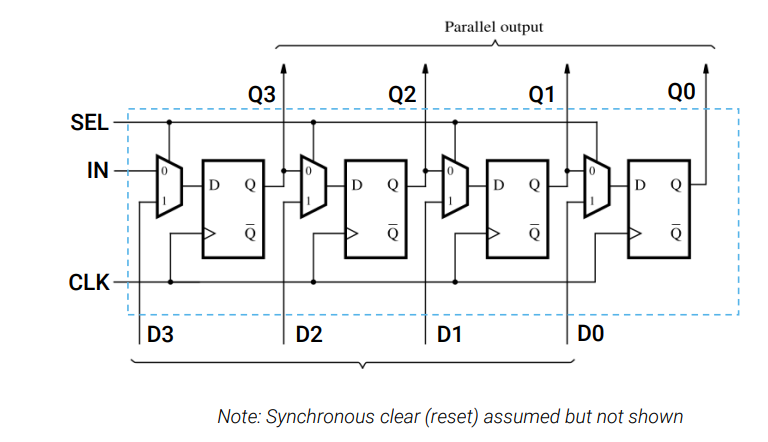
\includegraphics[scale=0.6]{52025-06-20.png}
    \end{center}
    The code is very similar to the one before expect that now we have another input $D$ a $n$ bit register and $SEL$ the selector. 
    \begin{lstlisting}
module shiftn (D, IN, SEL, CLR, CLK, Q);
    parameter n = 4;
    input [n-1:0] D;
    input IN, SEL, CLR, CLK;
    output reg [n-1:0] Q;

    integer k; // for loop iterator

    always @ (posedge CLK) 
    begin
    if (CLR == 1) Q <= 0;
    if (SEL == 1) Q <= D;
    else begin
        for (k = 0; k < n-1; k = k+1)
        begin
            Q[k] <= Q[k+1];
        end
        Q[n-1] <= IN;
    end
    end
endmodule
    \end{lstlisting}
    \begin{framedremark}
    Here, we use a for loop but this is equivalent to the concatenation we did before.
    \end{framedremark}
    
\end{parag}



\begin{parag}{Counter}
    Counter are simple circuits that increment or decrement their value\\
    \textbf{Applications}:
    \begin{itemize}
        \item Count the number of occurrences of certain events 
        \item  \textbf{Timers}: Generate timing intervals for controlling logic signals and, therefore managing the behavior of the circuit
        \item Keeping track of the time elapsed between events, in clock cycles
    \end{itemize}
    
    
\end{parag}



\begin{parag}{Counter up, with enable}
    The input of FFs are defined as:
    \begin{align*} 
        D_0 &= Q_0 \oplus EN\\
        D_1 &= Q_1 \oplus \left(Q_0 EN\right)\\
        D_2 &= Q_2 \oplus \left(Q_0Q_1 EN\right)\\
        D_3 &= Q_3 \oplus \left(Q_0Q_1Q_2 EN\right)\\
    \end{align*}
    More generally:
    \begin{align*} D_1 =  Q_i \oplus \left(\Pi_{k = 0}^{i-1}Q_k EN\right) \end{align*}
    This can only go up to $2^n$ after this it goes again to $0$ therefore it counts ``modulo $2^n$''.
    
    \begin{center}
        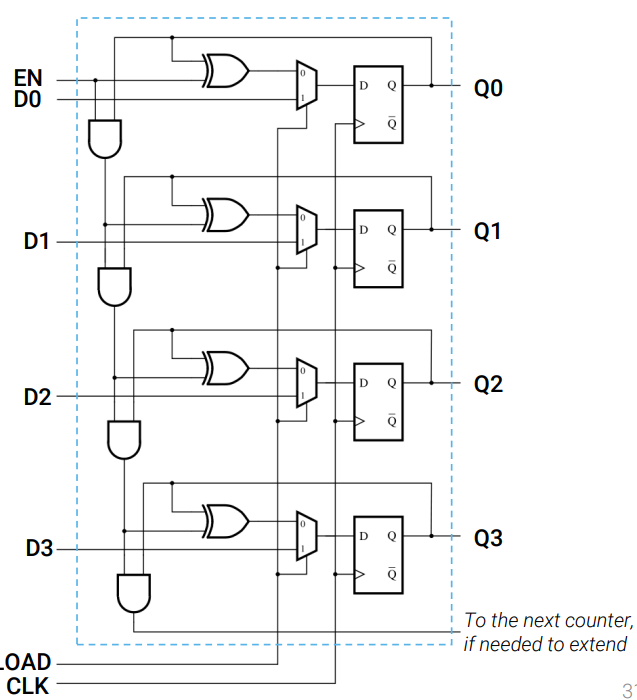
\includegraphics[scale=0.5]{62025-06-20.png}
    \end{center}
    
    Now if we want to implement this in verilog, it is very simple because we don't have to do any combinational logic:
    \begin{lstlisting}
module upcount (EN, CLR, CLK, Q);
    parameter n = 4;
    input EN, CLR, CLK;
    output reg [n-1:0] Q;

    always @ (posedge CLK)
    begin
        if (CLR == 1) Q <= 0;
        else if (EN == 1) Q = Q + 1;
    end
endmodule
    \end{lstlisting}
    
\end{parag}







\begin{parag}{Lecture- Digital logic and verilog, Part IX, Timing analysis of sequential circuit}
    I just put it there that I didn't do a summary of this lecture because there only a lot of schema and this is an algorithm to apply
    
\end{parag}
\begin{parag}{Timing analysis}
    In this slide
\end{parag}

\begin{parag}{$n-$to $-2^n$ binary decoder}
    A decoder (in short) is a logic circuit that receives an $n$-bit binary vector and produces an output vector of $2^n$ bits, in which all but one bit are logic zero\\
    Decoding the input: if $m$ is the unsigned decimal equivalent of the $n-$bits binary number at the input of the decoder, the output bit at \textbf{index} $ m$ will be set to logic $1$, all other output bits will be logic 0\\
    For instance if we take $n = 2$, we have that there is $2^2 = 4$ outputs. If we take for instance $\left(11\right)_2 = 3$ we have that the output is $1000$ the $y_3 = 1$:
    \begin{align*} 
        \left(w_1w_0\right) = \left(00\right) = \left(0\right) \to y_0 = 1 \to y = \left(0001\right)_2\\
        \left(w_1w_0\right) = \left(01\right) = \left(1\right) \to y_1 = 1\\
        \left(w_1w_0\right) = \left(10\right) = \left(2\right) \to y_2 = 1\\
        \left(w_1w_0\right) = \left(11\right) = \left(3\right) \to y_3 = 1 \to y = \left(1000\right)_2
    \end{align*}

We can make a truth table and then we will find:
\begin{align*} 
    y_0 &= \overline{w_1} \overline{w_0}\\
    y_1 &= \overline{w}_1w_0\\
    y_2 &= w_1 \overline{w}_0\\
    y_3 &= w_1w_0
\end{align*}
Which gives us the following circuit:
\begin{center}
    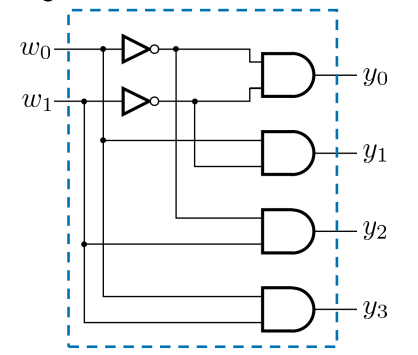
\includegraphics[scale=0.6]{72025-06-20.png}
\end{center}
\begin{framedremark}
Large decoder can be constructed with smaller one, for instance a $4$ to $16$ decoder can be constructed using $5$ decoder $2$ to $4$ with one at the root:
\begin{center}
    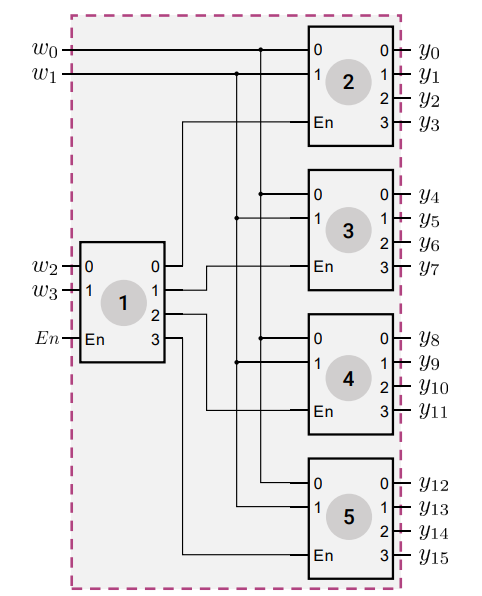
\includegraphics[scale=0.6]{82025-06-20.png}
\end{center}

\end{framedremark}

\end{parag}



\begin{parag}{Memory}
    We can seee memory as a two dimesnional array of $1$ bits memory elements (DFFs, latches, capacitors)\\
    One memory element $mem\left[i\right]$ where $i$ is the index of the \important{row} in the two dimensional array of bits, includes all bits in that row of the memory array and is typically referred to as one data \important{word}.\\
    \begin{itemize}
        \item In memory terminology, instead of  saying the index, we say \important{the adrdress} of the data word.
    \end{itemize}
\end{parag}
\begin{parag}{Memory access protocol}
    \begin{itemize}
        \item   \textbf{Synchronous write}: one the rising clock edge, if write enable (we) is active, memory \important{write} take place:
            \begin{align*} mem\left[addr\right] =  data\_in \end{align*}
            \item  \textbf{Asynchronous read}: at all times, memory \important{read} takes places:
                \begin{align*} data\_out =  meme\left[addr\right] \end{align*}
    \end{itemize}
    
    \begin{center}
        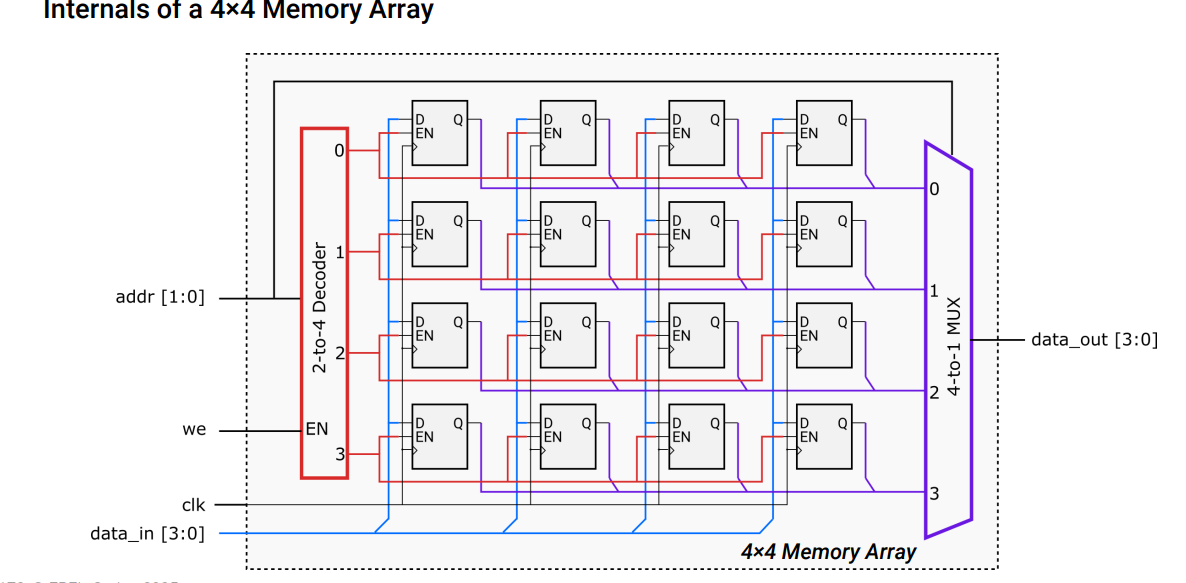
\includegraphics[scale=0.5]{92025-06-20.png}
    \end{center}
\end{parag}





\subsubsection{State Machines}
\begin{parag}{Finite state machine}
    \begin{itemize}
        Because circuits containing combinational and sequential logic have a state, we call them \textbf{state machines}
        \item States are represented by $n$ bit binary values (one memory element per one bit of the state)
            \begin{itemize}
                \item There are $2^n$ state possible that are representable with $n$ bits
            \end{itemize}
             \item as the number is limited (finite), we call such circuits \important{finite state machines (FSMs)}
    \end{itemize}
\end{parag}
\begin{parag}{Mealy State machine}
    \begin{definition}
    A finite state machine is a Mealy state machine if the output depend on the current state and current inputs.
    \end{definition}
\begin{center}
    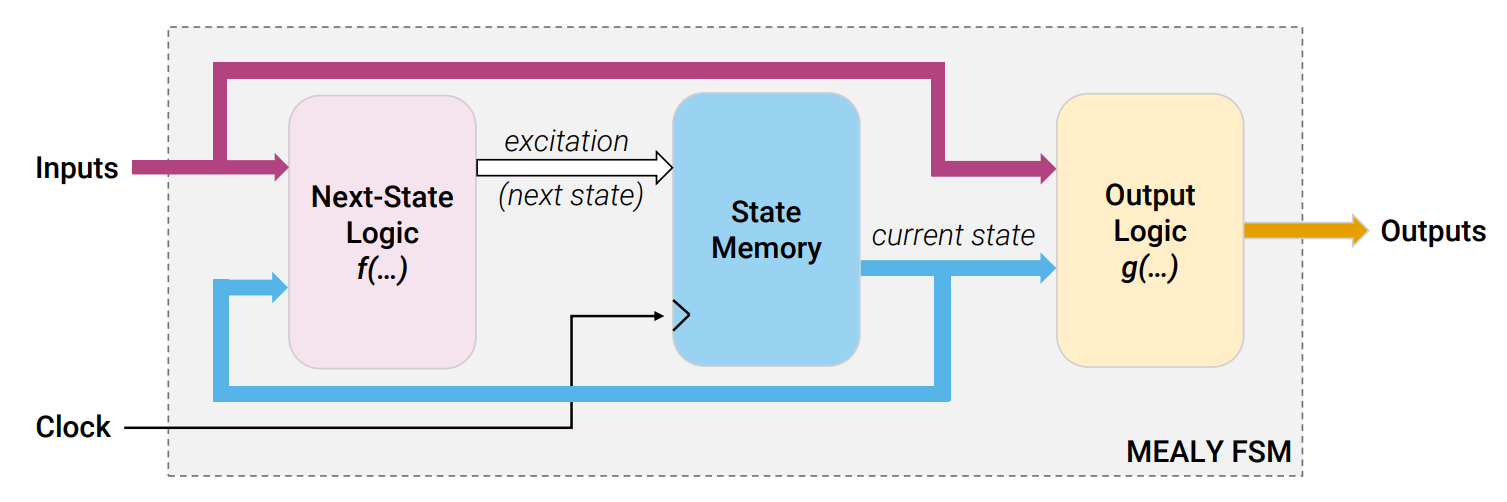
\includegraphics[scale=0.5]{102025-06-20.png}
\end{center}
\begin{itemize}
    \item The \textbf{state memory} is a set of $n$ flip flops that store the current state
        \begin{itemize}
            \item All connected to a common clock, causing them to update state once per clock period
        \end{itemize}
    \item The \textbf{next state} is a function of input and current state
        \begin{align*} \text{Next state } = f\left( \text{current state, input}\right) \end{align*}
    \item The \textbf{ output} is a function of the current state and inputs
        \begin{align*} \text{Output } = g\left(\text{current state, input}\right) \end{align*}
\end{itemize}
\end{parag}

\begin{parag}{Moore state machine}
    \begin{definition}
    A finite state machine is a \important{moore state machine} if the output depend on the current state only
    \end{definition}
    \begin{center}
        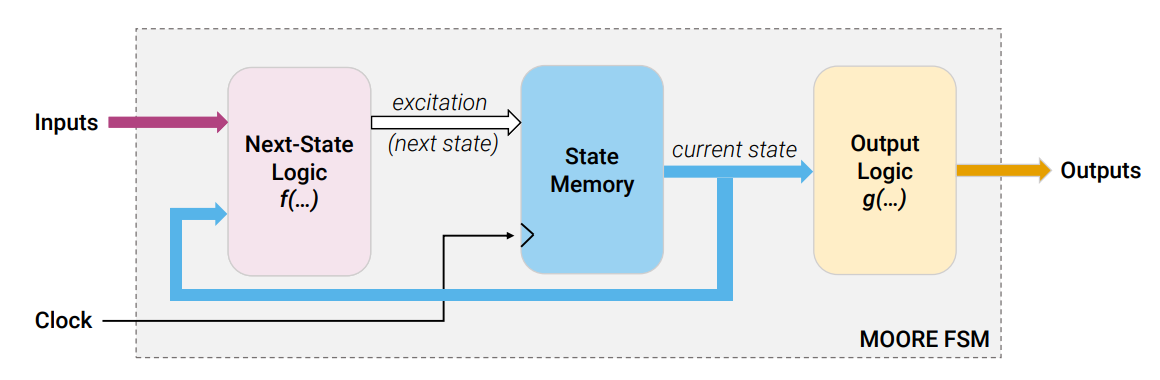
\includegraphics[scale=0.5]{112025-06-20.png}
    \end{center}
    \begin{itemize}
        \item The \textbf{next state} is a function of inputs and current state
            \begin{align*} \text{Next state } =  f\left(\text{current state, input}\right) \end{align*}
        \item The \textbf{output} is a function of the current state only
            \begin{align*} \text{Output} =  g\left(\text{current state}\right) \end{align*}
    \end{itemize}
    \begin{framedremark}
    Moore state machine are preferred (because there is no combinational path connecting inputs to outputs), whenever possible
    \end{framedremark}
    
    
    
\end{parag}


\begin{parag}{State machine analysis}
    Three basic steps:
    \begin{enumerate}
        \item Given a logic circuit, determine the next state and output function $f\left(\right), g\left(\right)$ respectively
        \item Use $f\left(\right)$ and $g\left(\right)$ to construct a \textbf{state/output table} that completely specifies the next state and the output of the circuit for every possible combination of current state and its inputs
        \item (optional) Draw a \textbf{state diagram} that presents the information from step $2$ in graphical form.
    \end{enumerate}
    
    
\end{parag}

\begin{parag}{State diagram}
    The explanation on how to do it is pretty good on the slide\\
    The next lecture have also very good example
    
\end{parag}
\begin{parag}{Bus}
    
    \begin{itemize}
        \item Digital systems are commonly composed of several modules exchanging data by means of a \textbf{ common } wires
        \item The shared set of wires is referred to as a \textbf{bus}
        \item Bus receives data from one or more brings it to the inputs of one or more modules
    \end{itemize}
    \begin{center}
        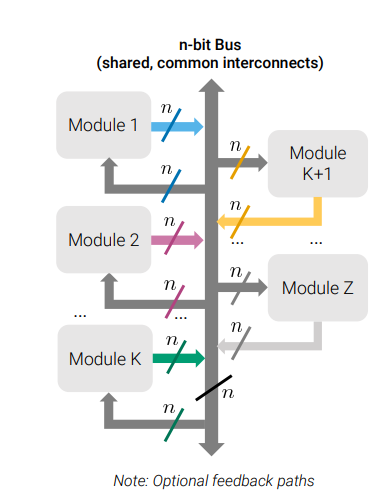
\includegraphics[scale=0.3]{122025-06-20.png}
    \end{center}
    
\end{parag}
\begin{parag}{Tri-state Drivers}
    \begin{center}
        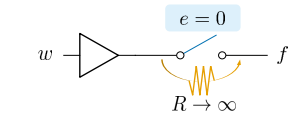
\includegraphics[scale=0.4]{132025-06-20.png}
    \end{center}
    \begin{center} \begin{tabular}{cc|c}$e$ & $w$ &  $z$\\  \hline 0& 0 &\textbf{Z}  \\  0& 1 &\textbf{Z}  \\ 1 & 0 & 0 \\  1& 1 &1  \end{tabular} \end{center} 
    When the enable input is inactive, the output is electrically disconnected from the data input; disconnected state is referred to as \important{high-impedance} state and usually denoted as \textbf{Z} or \textbf{z}
    \begin{itemize}
        \item Three states of a tre-state driver are logical $0$, logical $1$ and $z$  .
    \end{itemize}
    
\end{parag}
\begin{parag}{Bus with?}
    There is two possibility to build a bus, one is with tri state drivers and the other is with MUXes, we more generally implement Bus with MUXes
    
\end{parag}

















\subsection{Verilog}
\begin{parag}{Loops}
    Verilog  includes four types of loop statement
    \begin{itemize}
        \item \textbf{for}, \textbf{while} , \textbf{repeat} and \textbf{forever}
    \end{itemize}
    Logic synthesis tools typically support for loop:
    \begin{lstlisting}
for(initial index; terminal index;  increment)
begin
    statements;
end  
    \end{lstlisting}
    
    \begin{itemize}
        \item The \textbf{initial index} is evaluated once, before the first loop iteration
            \begin{itemize}
                \item Typically, it perfomrs the initialization of the integer loop control variable (e.g., $k = 0$)
            \end{itemize}
            \item In each loop iteration, the \textbf{begin-end} block is performed, and then the \textbf{increment} statement is evaluated (usaly $k = k+1$)
    \item Finally, the terminal index condition is checked
\begin{itemize}
    \item If true, another loop iteration is performed
    \item  if false, the loop terminates
    \item contrary to testing, for synthesis the terminal index condition has to compare the loop index to a \important{constant value}.
\end{itemize}

    \end{itemize}
    
\end{parag}
\begin{parag}{Scalar signal values}
    Verilog supports one bit signals (scalars) and vectors. Each individual signal can have one of the four values:
    \begin{center} \begin{tabular}{cc} \hline Value & Meaning \\ \hline $0$ & logic value $0$ \\ 1 & logic value $1$ \\ $z$ & or $Z$, tri-state (high-impedance) \\ $x$ &  or $X$, unknown value or don't care \end{tabular} \end{center} 
    
\end{parag}
\begin{parag}{Logic operator}
    used the same way as we used them in java, c++ etc...
    \begin{center} \begin{tabular}{c|c}== & logic equality \\ != & logical inequality \\ \&\& & logical and \\ $\left|\right|$ & logic or \\ ! & logical not \end{tabular} \end{center} 
\end{parag}

\begin{parag}{Equality}
    \begin{itemize}
        \item Equality operators compare operands bit for bit
        \item The result is $0$ if comparison fails and $1$ otherwise
    \end{itemize}
    \begin{center} \begin{tabular}{cc}$a = = b$ equality & $a$ equal $b$, result can be unknown \\ $a $!=  $b$ inequality & a not equal to $b$, result can be unknown \\$a = = = b$ case equality  & $a$ equal to $b$, including $z$ and $x$ \\ $a$ !=== $b$ case inequality & a not equal to b, including $x$ and $z$ \end{tabular} \end{center} 
    
    
\end{parag}




\subsubsection{Arrays}
\begin{parag}{Two-Dimensional arrays}
    In verilog, we can declare two dimensional arrays, an array $mem$ of $Ndw$ data words, where each word has $Ndb$ bits is declared as
    \begin{lstlisting}
        reg[Ndb-1:0] mem [Ndw-1:0];
    \end{lstlisting}
    
    For instance creating
    \begin{lstlisting}
        reg [7:0] mem [3:0];
    \end{lstlisting}
   create a array of length $4$ where the elements of the array are of length $8$, this is a array of byte of length $4$.
    
    
\end{parag}




\begin{parag}{Parameterized Verilog module}
    In verilog, we can override parameter (which where considered comme constante) when using it from another module.\\
    Imagine we create a function $f\left(x\right)$ which have a parameter $n$ in it. If we want to use $f$ but we another $n$ then we can just change it like it is a parameter of the function itself
    \begin{lstlisting}
        f #(.n(3)) f1 (.x(oui));
    \end{lstlisting}

    
\end{parag}



\begin{parag}{Verilog conditional operator}
    Same as in Java:
    \begin{lstlisting}
        A ? B : C
    \end{lstlisting}
    
\end{parag}

\begin{parag}{Reduction Operators}
    Reduction operators are unary operators (take one operand) that perform bitwise operations on all bits of the vector operand to produces a single bit result
    \begin{center} \begin{tabular}{cc}\hline \& & reduction and \\ $\sim$\&  & reduction nand  \\ | &reduction or  \\ $\sim$ |  & reduction nor \\ $\hat{}$ & reduction xor \\$\sim \hat{}$  & reduction xnor \end{tabular} \end{center} 
\end{parag}
\begin{parag}{Why is it useful?}
\begin{itemize}
    \item Zero detection - check if any bit of a bus vector is $1$ without a loop
        \begin{lstlisting}
            wire zero = ~| my_bus; // the tilde is a bit too high
        \end{lstlisting}
    \item Parity checking - simple error detection (for memory communication buses) wire
        \begin{lstlisting}
            parity = ^data // Cor all bits for parity
        \end{lstlisting}
    \item Fast flag setting - a equick way to set a ``done'' flag if any several modules have completed
        \begin{lstlisting}
            wire done = | done_signals;
        \end{lstlisting}
    \item Checking ``all ones'' quickly (e.g. completion/done flags, timers, etc.)
        \begin{lstlisting}
            wire all_ones = & status_bits;
        \end{lstlisting}
        
\end{itemize}

    
\end{parag}



\begin{parag}{Generate construct}
    Combination of for loops with module instantiations.\\
    Verilog \textbf{generate} construct allows module instantiation to be included inside \important{for} loops and \important{if-else} statements
    \begin{itemize}
        \item \important{generate} construct lets us create multiple instances (loops, or conditionally included) of hardware at compile time - cleanly and systematically- without manually copying code (repetitive, harder maintenance) and introducing errors (esp. when scaling the design)
        \item \important{generate} provides a way to create mutliple pieces of hardware bases on parameters or iterations
        \item If a \important{for} loop is included in the \textbf{generate} block, the loop index variable has to be of type \important{genvar}.
        \item \important{genvar} is an integer variable that can only have values $\geq 0$, (it would not make sens to instantiate a negative number of modules) and can only be used inside generate blocks
    \end{itemize}
    For instance (there is not the entire code but this is the idea):
    \begin{lstlisting}
        // generate block
        generate      // optional keyword, helps readability
            for (g = 0; g < n ; g = g + 1) 
            begin
                fulladd stage (.a(A[g], .b(B[g]) ... )
            end
        endgenerate // optional keyword, helps readability
    \end{lstlisting}
    Here:
    \begin{itemize}
        \item \important{fulladd} is the name of the module being instantiated multiple times
        \item \important{stage} is the name of one instance of a module; it is used defined, so choose an appropriate one
    \end{itemize}
    
\end{parag}




\subsubsection{Processor}


A processor is divided into two parts
\begin{parag}{Part $I$}
        It concerns everything related to data:
        \begin{itemize}
            \item Variable storage/read/write
            \item Operations on variables
            \item Includes the digital logic circuits that perform operations on data or hold data
        \end{itemize}
        It \important{contains}:
        \begin{itemize}
            \item an arithmetic logic unit (ALU)
            \item A register file
        \end{itemize}
        \begin{subparag}{ALU}
            The \important{ALU} performs the operations on program variables (e.g. bitwise, logic, shift comparisons etc...)
            \begin{center}
                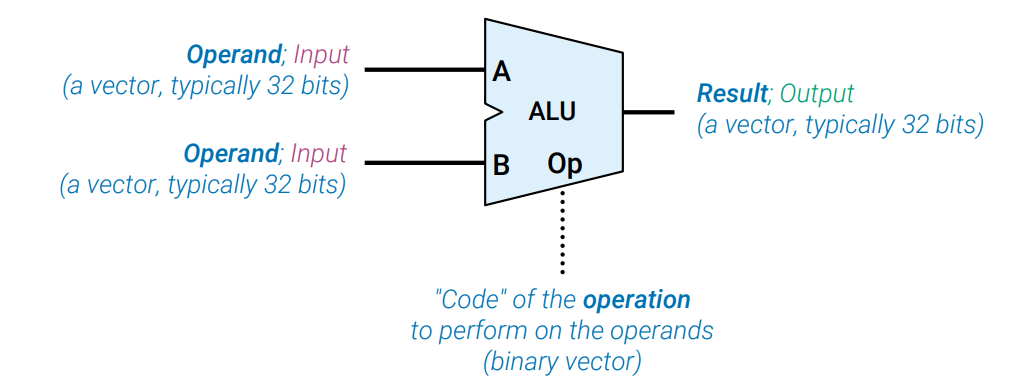
\includegraphics[scale=0.6]{142025-06-20.png}
            \end{center}
            
        \end{subparag}
        \begin{subparag}{Register file}
            \important{register file} is an array of registers for keeping the program variables and some other special uses.
            \begin{center}
                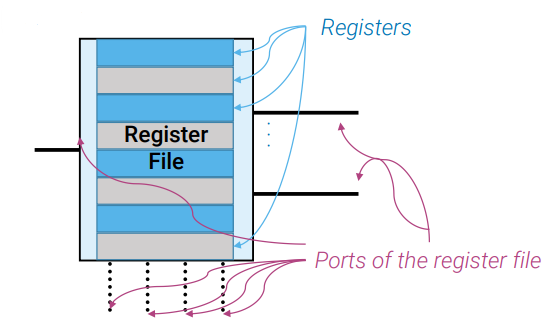
\includegraphics[scale=0.5]{152025-06-20.png}
            \end{center}
            \begin{itemize}
                \item Two registers can be read in the same clock cycle
                \item Reading from and writing to registers is fast (one CPU clock cycle)
                \item FF is expensive per bit
                    \begin{itemize}
                        \item DFF typically contains $\sim 20$ transistors
                    \end{itemize}
                    \item  in practice register files are constructed using SRAM memory cells
            \end{itemize}
            
        \end{subparag}
       \begin{center}
           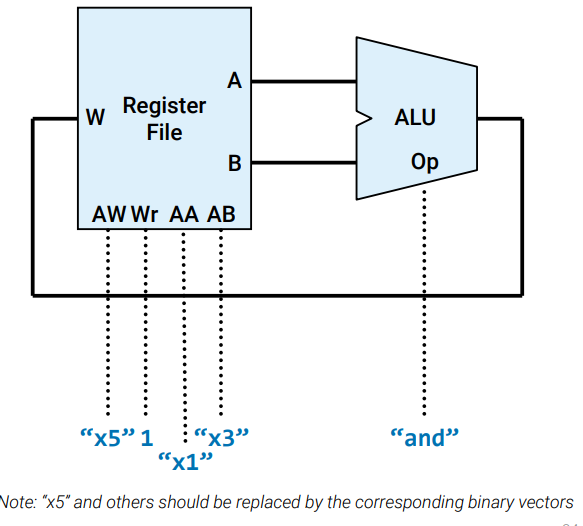
\includegraphics[scale=0.7]{162025-06-20.png}
       \end{center}
       Let us denote what everything means:
           \begin{itemize}
               \item W $\to$ Data to write to register ``AW'' (a vector, typically 32 bits); inputs
               \item AW $\to$ index of the register ``AW'' to write to (or adress)
               \item Wr $\to$ Write enable - if active, data on input $W$ port is written to register AW; input
               \item AA $\to$ Index of the register $A$
               \item AB $\to$ index of register $B$
               \item A $\to$ Data from register $A$
               \item B $\to$ data from register $B$
           \end{itemize}
           When there are all connected as in the figure we have that:
           \begin{itemize}
               \item ALU receives operands from the outputs of the register file
               \item Register file receives the result of the operation performed by the ALU and saves it in one of its registers
               \item Registers in the register file and the ALU are tightly coupled (i.e. close, wires connecting them are short), which  make data transfer between them \textbf{fast}
           \end{itemize}
           
           
       
        

        
\end{parag}


\begin{parag}{Part $II$: Control Path}
        This one concerns everything related to the code exectuion
        \begin{itemize}
            \item instruction reading/decoding/sequencing
            \item  Manages the digital circuits of the datapath so they perform the operations as specified by the instructions
        \end{itemize}
        \begin{subparag}{Roles}
            \begin{itemize}
                \item Instruction reading (loading instructions from the program in memory)
                \item Sequencing instructions (ensuring the correct program order)
                \item Decoded the instruction from its binary form
                \begin{itemize}
                    \item Depending on the instruction, set controls signals for the ALU and the register File accordingly
                \end{itemize}
            \item Implements the finite state machine of the processor
            \end{itemize}
            
        \end{subparag}
        
        
\end{parag}

\begin{parag}{Instruction memory}
    The question is where is the program?
    \begin{itemize}
        \item The program (instructions) resided in a larger memory external to the CPU
    \end{itemize}
    We call this memory \textbf{instruction memory}
    \begin{itemize}
        \item \textbf{External} to the processor
        \item Typically made from SRAM memory cells
    \end{itemize}
    \begin{framedremark}
        \begin{center}
            Instruction memory $\neq$ Register file
        \end{center}
    \end{framedremark}
    The CPU has an additional register dedicated to keeping the adress (location) of the instruction in memory
    \begin{center}
        \textbf{Program Counter (PC)}
    \end{center}
    \begin{itemize}
        \item Control logic updates the program counter (PC), in preparation for reading of the \textbf{next} instruction
    \end{itemize}
    
    
    \begin{center}
        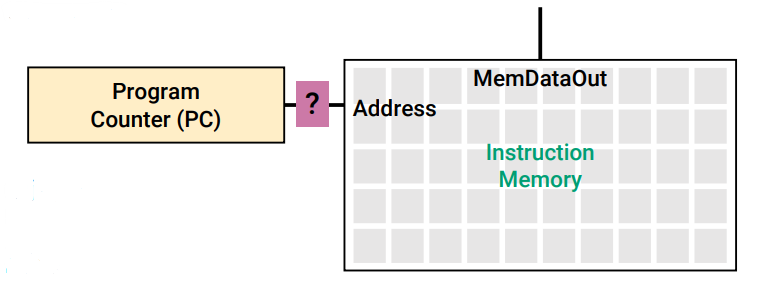
\includegraphics[scale=0.6]{172025-06-20.png}
    \end{center}
    \begin{itemize}
        \item The next instruction in memory is typically at the neighboring memory address, higher than the previous
            \begin{itemize}
                \item PC should be incremented to ``point'' to the next instruction 
            \end{itemize}
    \end{itemize}
    

\end{parag}
\begin{parag}{Finally}
    Once the instruction is read from the instruction memory, it must be \textbf{decoded}\\
    Decoding is \textbf{parsing} the binary representation of the instruction, to \textbf{identify} all the relevant info:
    \begin{itemize}
        \item operation
        \item destination
        \item operands
    \end{itemize}
    \begin{center}
        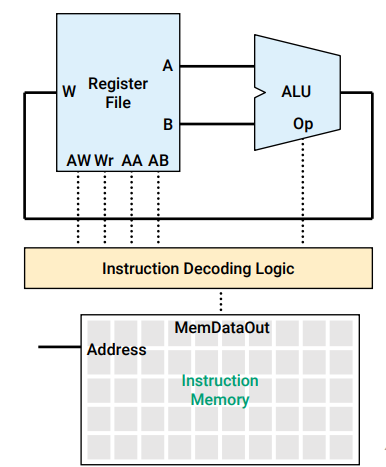
\includegraphics[scale=0.4]{182025-06-20.png}
    \end{center}
\end{parag}
\begin{parag}{Type of computer architecture}
    \begin{itemize}
        \item \textbf{Harvard} architecture
            \begin{itemize}
                \item Instructions and data memory reside in \textbf{separate} memories
            \end{itemize}
        \item \textbf{Von Neuman} architecture
            \begin{itemize}
                \item Instructions and data reside in the \textbf{same} memory
                \item We say the memory is \textbf{unified}
                \item In general purpose computers (desktops, laptops, servers, etc...) Von Neumann architecture is \textbf{predominant}.
            \end{itemize}
            
    \end{itemize}
    
\end{parag}

\begin{parag}{Riscv summary (executive summary)}
    \begin{itemize}
        \item \textbf{Assembly} language is the last human readable level of code
        \item Below assembly is only the machine code (binary)
        \item CPU instructions are kept in the instruction memory, which is different from the register file
        \item In Von Neuman computer architecture, instruction and data memories are unified
        \item Instruction are \textbf{encoded} as binary data words, and oftern contain the type of operation, the sources (operands) and the destination (result)
        \item \textbf{Instruction set architecture (ISA)} is one of the important \important{abstraction} in computing
        \item ISA refers to the set of instructions that a CPU can execute and the programming model that these instructions define for software developers
    \end{itemize}
    
\end{parag}
\begin{parag}{Memory}
    \begin{itemize}
        \item Memory is \important{byte-adressable}, meaning that one address corresponds to one byte (therefore if you want to do a loop over word you have to add 4 not 1)
        \item Therefore the program counter is always adding $4$ by $4$ (apart from jumps)
    \end{itemize}
    
\end{parag}

\begin{parag}{Byte Ordering}
    \begin{subparag}{Little-endian}
        The least significant bits of the word (byte $B_0$, the one at the ``little'' end of the word) is at the lowest memory address
    \end{subparag}
    \begin{subparag}{Big-endian}
        The most significant bits of the word (byt $B_3$, the one at the ``BIG'' end of the word) is at the lowest memory address)
    \end{subparag}
\end{parag}


\paragraph{CPU Performance}


\begin{parag}{CPU Time}
    \begin{definition}
    The time the CPU spends on our program\\
    Ignore overheads, such as the time to read/write to input/output devieces, and performing unrelated system tasks.
    \end{definition}
    We measure time in decrete time intervals, \textbf{clock cycles}

    \begin{align*} t_{CPU} = \frac{CPU_{cycles}}{\nu_{CLK}} \end{align*}
    We also have the 
    \begin{align*} CPU_{cycles} = \text{Instructions for a program} \cdot  \text{average clock cycles per instruction} \end{align*}
\end{parag}
\begin{parag}{Factors impacting program performance}
    The algorithm determines the number of instructions executed. It may affect CPI as well, favoring slower or faster instructions\\
    Also, ISA impact performance, it affects all three aspects of CPU performances: the instructions needed to perform the required function, the cost in cycles of each instruction, and the CPU clock rate.
    
\end{parag}


\begin{parag}{Performance and power}
    An increase in clock rate brings improvement in performance, but it also increase power dissipation\\
    The power dissipation in CMOS logic gates, as a function of switching frequency, capacitive load, and power supply:
    \begin{align*} P_D =   fCV^2 \end{align*}
\end{parag}























